\documentclass[11pt,a4paper]{article}
\usepackage[utf8]{inputenc}
\usepackage[english]{babel}
\usepackage[T1]{fontenc}
\usepackage{amsmath}
\usepackage{amsfonts}
\usepackage{amssymb}
\usepackage{graphicx}
\usepackage{array}
\usepackage{multirow}
\usepackage[left=2cm,right=2cm,top=2cm,bottom=2cm]{geometry}
\author{Guillem Tocabens}
\title{First measurements}
\begin{document}

\section{Setup}

For these measurements, we used two different setups, the main difference between the two being the absence, or not, of a lead shielding to perform the measurements. The setup with the shielding is given in Figure~\ref{Setup}.

\begin{figure}[!h]
\centering
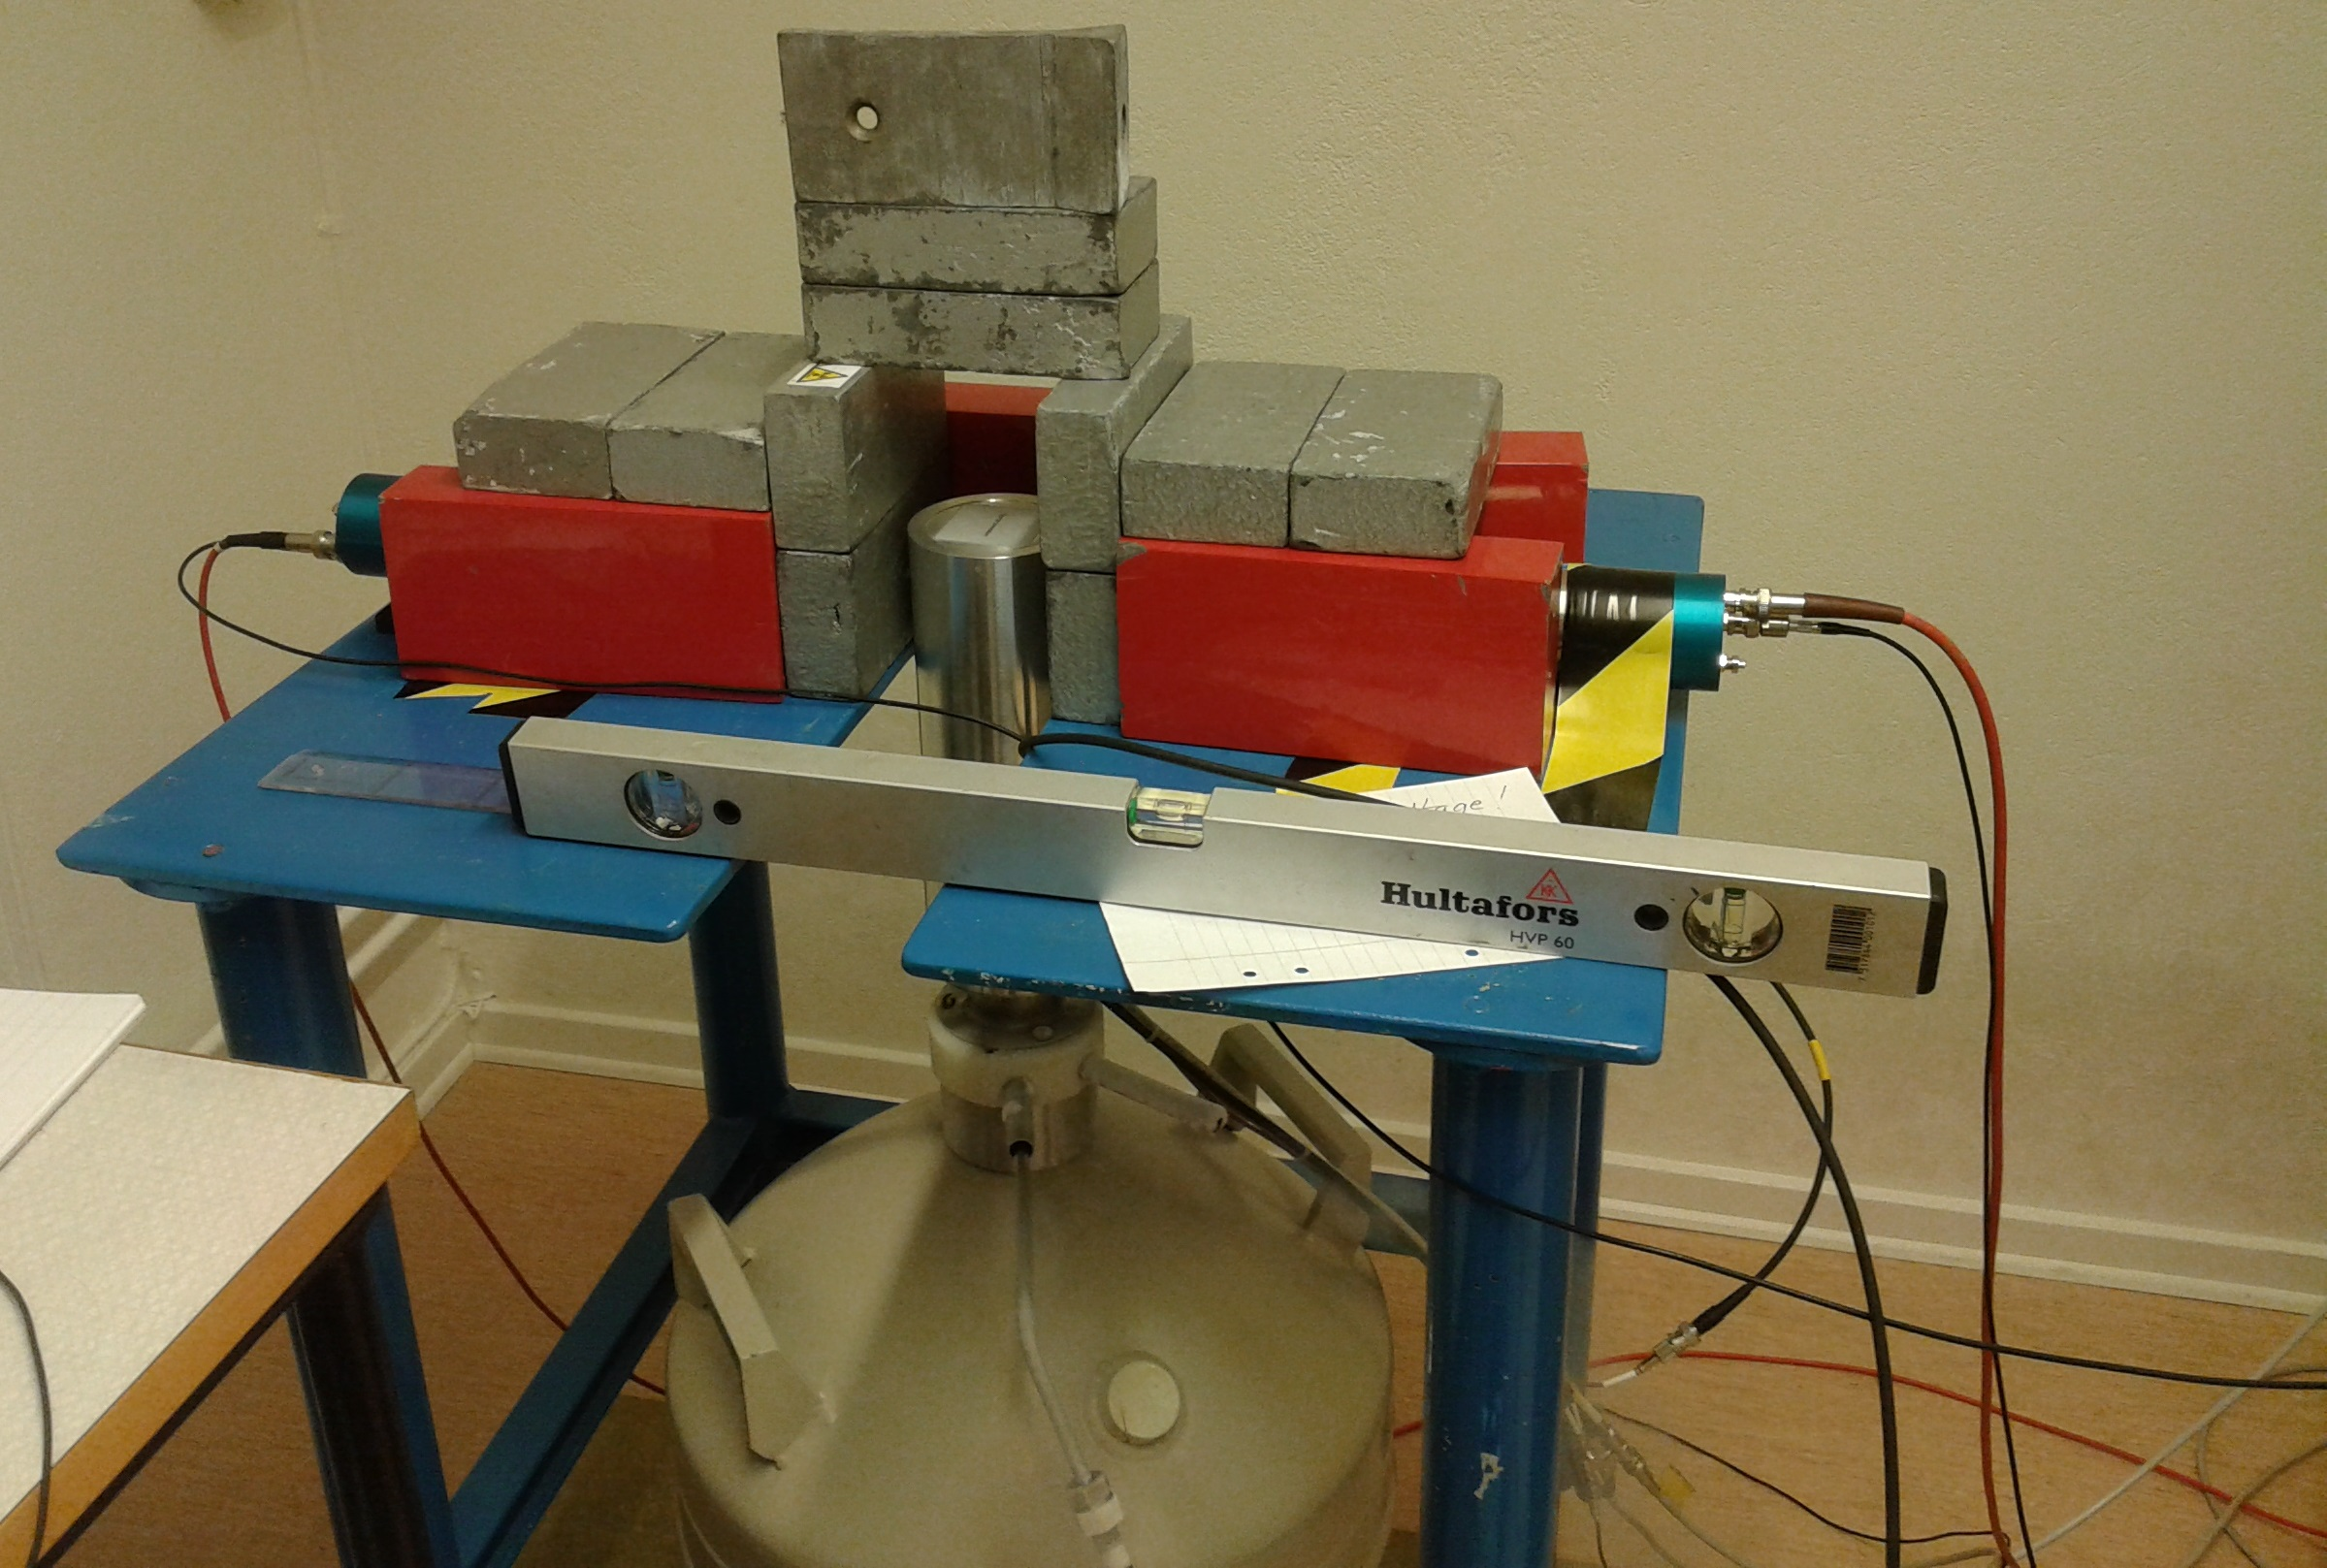
\includegraphics[scale=0.2]{Setup.jpg}
\caption{Picture of the original setup (with the lead shielding).}
\label{Setup}
\end{figure}

The germanium detector is placed in the bottom of the setup, and the radioactive source is placed above (on the blue table on the picture). The beam is collimated through two brics of lead containing a hole of 10mm diameter and the source is around 202mm above the top of the cryostat (thus 207mm from the top of the crystal). On the sides of the germanium detector are placed two scintillators that will be used to measure coincidences. The whole setup is shielded by lead bricks in order to avoid noise. In the second setup that we used, the source is held by a metallic arm, roughly at the same distance from the top of the crystal and we removed all the lead bricks to measure the peak-to-Compton ratio and the efficiency of the detector.

For these first measurements, we used two sources, one source of Cobalt 60 to perform the calibration, and a source of Cesium 137. The activities of the sources are, respectively, 370kBq and 16.5kBq. %to calculate with the ages of the sources
Both setups were used with both sources and the measurements last until the net area of the biggest peak in the spectrum was 100000 counts at least, to get proper statistics.



\end{document}